\definecolor{chinese}{rgb}{0, 1, 0} %chinese 
\definecolor{english}{rgb}{0, 0, 1}%english 
\definecolor{french}{rgb}{.8, 0, 0}%french 
\definecolor{german}{rgb}{.5, .5, .5}%german 
\definecolor{japanese}{rgb}{0, 0, .5}%japanese 
\definecolor{russian}{rgb}{0, .5, 0}%russian 
\definecolor{spanish}{rgb}{.20, .92, .85}%spanish 


\begin{figure}[h]
\centering

        \begin{tikzpicture}
        \begin{scope}[xshift=1.5cm]
            \node[anchor=south west,inner sep=0] (image) at (0,0)
            {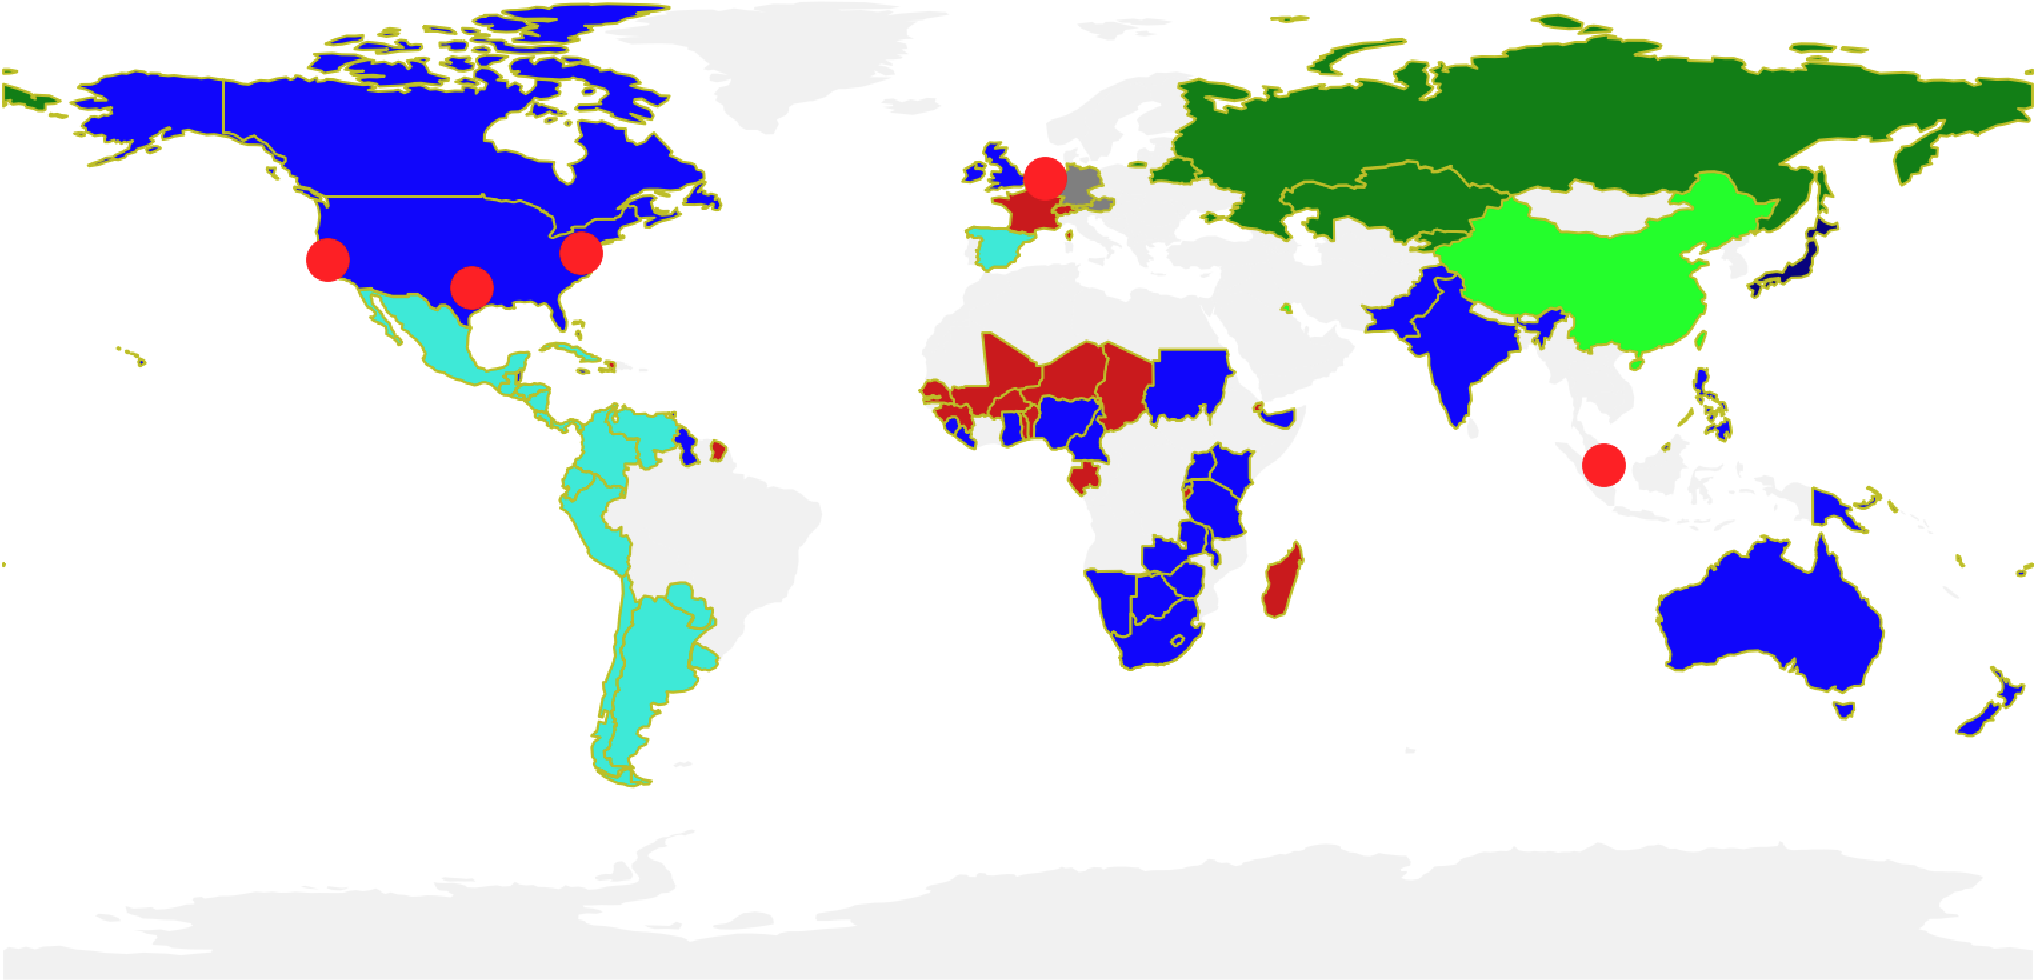
\includegraphics[width=1\textwidth]{embodied_cost_model/images/worldmap_4.png}};
        \end{scope}
        
        \begin{scope}[xshift=1.0cm]
            \node [anchor=center] (chinese) at (2,-.6) {\small{Chinese}};
            \filldraw[outer color=chinese, inner color=chinese] (1.8,-.4) rectangle (2.2,0); % chinese
            
            \node [anchor=center] (english) at (4,-.6) {\small{English}};
            \filldraw[outer color=english, inner color=english] (3.8,-.4) rectangle (4.2,0); % english
            
            \node [anchor=center] (french) at (6,-.6) {\small{French}};
            \filldraw[outer color=french, inner color=french] (5.8,-.4) rectangle (6.2,0); % french
            
            \node [anchor=center] (german) at (8,-.6) {\small{German}};
            \filldraw[outer color=german, inner color=german] (7.8,-.4) rectangle (8.2,0); % german
            
            \node [anchor=center] (japanese) at (10,-.6) {\small{Japanese}};
            \filldraw[outer color=japanese, inner color=japanese] (9.8,-.4) rectangle (10.2,0); % japanese
            
            \node [anchor=center] (russian) at (12,-.6) {\small{Russian}};
            \filldraw[outer color=russian, inner color=russian] (11.8,-.4) rectangle (12.2,0); % russian
            
            \node [anchor=center] (spanish) at (14,-.6) {\small{Spanish}};
            \filldraw[outer color=spanish, inner color=spanish] (13.8,-.4) rectangle (14.2,0); % spanish
            
            \node [anchor=center] (dc_location) at (9,-1.1) {\small{Data Center Locations}};
            \filldraw[red] (7,-1.1) circle (4pt); 
            
            \end{scope}
            
        \end{tikzpicture}

\caption[Source country of language and DC locations]{Source country of language and DC locations map.}
\label{image:world_language_map}
\end{figure}